%%%%%%%%%%%%%%%%%%%%%%%%%%%%%%%%%%%%%%%%%
% Beamer Presentation
% LaTeX Template
% Version 2.0 (March 8, 2022)
%
% This template originates from:
% https://www.LaTeXTemplates.com
%
% Author:
% Vel (vel@latextemplates.com)
%
% License:
% CC BY-NC-SA 4.0 (https://creativecommons.org/licenses/by-nc-sa/4.0/)
%
%%%%%%%%%%%%%%%%%%%%%%%%%%%%%%%%%%%%%%%%%

%----------------------------------------------------------------------------------------
%	PACKAGES AND OTHER DOCUMENT CONFIGURATIONS
%----------------------------------------------------------------------------------------

\documentclass[
	11pt, % Set the default font size, options include: 8pt, 9pt, 10pt, 11pt, 12pt, 14pt, 17pt, 20pt
	%t, % Uncomment to vertically align all slide content to the top of the slide, rather than the default centered
	%aspectratio=169, % Uncomment to set the aspect ratio to a 16:9 ratio which matches the aspect ratio of 1080p and 4K screens and projectors
]{beamer}
\setcounter{tocdepth}{5}
\graphicspath{{Images/}{./}} % Specifies where to look for included images (trailing slash required)

\usepackage{booktabs} % Allows the use of \toprule, \midrule and \bottomrule for better rules in tables
%----------------------------------------------------------------------------------------
%	SELECT LAYOUT THEME
%----------------------------------------------------------------------------------------

% Beamer comes with a number of default layout themes which change the colors and layouts of slides. Below is a list of all themes available, uncomment each in turn to see what they look like.
\usepackage{tikz}
\usepackage{pgfplots}
\pgfplotsset{compat=1.18}
\usepackage{wrapfig}
\usepackage{graphicx}
%\usetheme{default}
%\usetheme{AnnArbor}
%\usetheme{Antibes}
%\usetheme{Bergen}
%\usetheme{Berkeley}
%\usetheme{Berlin}
%\usetheme{Boadilla}
%\usetheme{CambridgeUS}
%\usetheme{Copenhagen}
%\usetheme{Darmstadt}
%\usetheme{Dresden}
%\usetheme{Frankfurt}
%\usetheme{Goettingen}
%\usetheme{Hannover}
%\usetheme{Ilmenau}
%\usetheme{JuanLesPins}
%\usetheme{Luebeck}
\usetheme{Madrid}
%\usetheme{Malmoe}
%\usetheme{Marburg}
%\usetheme{Montpellier}
%\usetheme{PaloAlto}
%\usetheme{Pittsburgh}
%\usetheme{Rochester}
%\usetheme{Singapore}
%\usetheme{Szeged}
%\usetheme{Warsaw}

%----------------------------------------------------------------------------------------
%	SELECT COLOR THEME
%----------------------------------------------------------------------------------------

% Beamer comes with a number of color themes that can be applied to any layout theme to change its colors. Uncomment each of these in turn to see how they change the colors of your selected layout theme.

%\usecolortheme{albatross}
%\usecolortheme{beaver}
%\usecolortheme{beetle}
%\usecolortheme{crane}
%\usecolortheme{dolphin}
%\usecolortheme{dove}
%\usecolortheme{fly}
%\usecolortheme{lily}
%\usecolortheme{monarca}
%\usecolortheme{seagull}
%\usecolortheme{seahorse}
%\usecolortheme{spruce}
%\usecolortheme{whale}
%\usecolortheme{wolverine}

%----------------------------------------------------------------------------------------
%	SELECT FONT THEME & FONTS
%----------------------------------------------------------------------------------------

% Beamer comes with several font themes to easily change the fonts used in various parts of the presentation. Review the comments beside each one to decide if you would like to use it. Note that additional options can be specified for several of these font themes, consult the beamer documentation for more information.

\usefonttheme{default} % Typeset using the default sans serif font
%\usefonttheme{serif} % Typeset using the default serif font (make sure a sans font isn't being set as the default font if you use this option!)
%\usefonttheme{structurebold} % Typeset important structure text (titles, headlines, footlines, sidebar, etc) in bold
%\usefonttheme{structureitalicserif} % Typeset important structure text (titles, headlines, footlines, sidebar, etc) in italic serif
%\usefonttheme{structuresmallcapsserif} % Typeset important structure text (titles, headlines, footlines, sidebar, etc) in small caps serif

%------------------------------------------------

%\usepackage{mathptmx} % Use the Times font for serif text
\usepackage{palatino} % Use the Palatino font for serif text

%\usepackage{helvet} % Use the Helvetica font for sans serif text
\usepackage[default]{opensans} % Use the Open Sans font for sans serif text
%\usepackage[default]{FiraSans} % Use the Fira Sans font for sans serif text
%\usepackage[default]{lato} % Use the Lato font for sans serif text

%----------------------------------------------------------------------------------------
%	SELECT INNER THEME
%----------------------------------------------------------------------------------------

% Inner themes change the styling of internal slide elements, for example: bullet points, blocks, bibliography entries, title pages, theorems, etc. Uncomment each theme in turn to see what changes it makes to your presentation.

%\useinnertheme{default}
\useinnertheme{circles}
%\useinnertheme{rectangles}
%\useinnertheme{rounded}
%\useinnertheme{inmargin}

%----------------------------------------------------------------------------------------
%	SELECT OUTER THEME
%----------------------------------------------------------------------------------------

% Outer themes change the overall layout of slides, such as: header and footer lines, sidebars and slide titles. Uncomment each theme in turn to see what changes it makes to your presentation.

%\useoutertheme{default}
%\useoutertheme{infolines}
%\useoutertheme{miniframes}
%\useoutertheme{smoothbars}
%\useoutertheme{sidebar}
%\useoutertheme{split}
%\useoutertheme{shadow}
%\useoutertheme{tree}
%\useoutertheme{smoothtree}

%\setbeamertemplate{footline} % Uncomment this line to remove the footer line in all slides
%\setbeamertemplate{footline}[page number] % Uncomment this line to replace the footer line in all slides with a simple slide count

%\setbeamertemplate{navigation symbols}{} % Uncomment this line to remove the navigation symbols from the bottom of all slides

%----------------------------------------------------------------------------------------
%	PRESENTATION INFORMATION
%----------------------------------------------------------------------------------------

\title[Anw. h\"ohere Mathe]{Anwendung Höherer Mathematik} % The short title in the optional parameter appears at the bottom of every slide, the full title in the main parameter is only on the title page

%\subtitle{Optional Subtitle} % Presentation subtitle, remove this command if a subtitle isn't required

\author[]{Sebastian Matkovich} % Presenter name(s), the optional parameter can contain a shortened version to appear on the bottom of every slide, while the main parameter will appear on the title slide

\institute[FHCW]{FH Campus Wien \\ \smallskip \textit{sebastianmatkovich@gmail.com}} % Your institution, the optional parameter can be used for the institution shorthand and will appear on the bottom of every slide after author names, while the required parameter is used on the title slide and can include your email address or additional information on separate lines

\date[\today]{ \today} % Presentation date or conference/meeting name, the optional parameter can contain a shortened version to appear on the bottom of every slide, while the required parameter value is output to the title slide

%----------------------------------------------------------------------------------------

\begin{document}

%----------------------------------------------------------------------------------------
%	TITLE SLIDE
%----------------------------------------------------------------------------------------

\begin{frame}
	\titlepage % Output the title slide, automatically created using the text entered in the PRESENTATION INFORMATION block above
\end{frame}

%----------------------------------------------------------------------------------------
%	TABLE OF CONTENTS SLIDE
%----------------------------------------------------------------------------------------

% The table of contents outputs the sections and subsections that appear in your presentation, specified with the standard \section and \subsection commands. You may either display all sections and subsections on one slide with \tableofcontents, or display each section at a time on subsequent slides with \tableofcontents[pausesections]. The latter is useful if you want to step through each section and mention what you will discuss.

\begin{frame}
%	\frametitle{Presentation Overview} % Slide title, remove this command for no title
	
	\tableofcontents % Output the table of contents (all sections on one slide)
%	\tableofcontents[pausesections] % Output the table of contents (break sections up across separate slides)
\end{frame}

%----------------------------------------------------------------------------------------
%	PRESENTATION BODY SLIDES
%----------------------------------------------------------------------------------------

%\section{Wiederholung Differenzialrechnung Integralrechnung} % Sections are added in order to organize your presentation into discrete blocks, all sections and subsections are automatically output to the table of contents as an overview of the talk but NOT output in the presentation as separate slides
%
%%------------------------------------------------
%\begin{frame}
%	\frametitle{Differenzialrechnung}
%	Die Ableitung einer Umkehrfunktion $f^{-1}(y)=x(y)$ erhalten wir ganz leicht \"uber die Leibnizschreibweise folgenderma\ss en:
%	\begin{equation}
%		\frac{dx}{dy}=\frac{1}{\frac{dy}{dx}}
%	\end{equation}
%	Ein einfaches Beispiel, das h\"aufig bei Differenzialgleichungen auftritt, bei denen die Ableitung dieser Funktion integriert wird ist ln(x).
%	\begin{equation}
%		\frac{d\ln(y)}{dy}=\frac{1}{\frac{de^x}{dx}}=\frac{1}{e^x}=\frac{1}{y}
%\end{equation}
%	\frametitle{Differenzialrechnung}
%	Damit ist das h\"aufig bei Differenzialgleichungen auftretende Integral\"uber \frac{1}{x}:
%	\begin{equation}
%		\int{\frac{1}{x}}{dx}=\log{x} 
%	\end{equation}
%\end{frame}
\section{Wiederholung Differenzial-/ Integralrechnung}
\subsection{Differenzialrechnung}
\begin{frame}
	\frametitle{Differenzialrechnung}
	Die Ableitung der Exponentialfunktion l\"asst sich so herleiten:
	\begin{equation}
		e = \lim_{n \rightarrow \infty} \left(1 + \frac{1}{n}\right)^n = \lim_{h \rightarrow 0} \left(1 + h\right)^{\frac{1}{h}}
	\end{equation}
	\begin{equation}
		\frac{de^x}{dx}=\lim_{h \rightarrow 0} \frac{e^{x+h}-e^x}{h} = e^x\cdot\lim_{h \rightarrow 0} \frac{e^h-1}{h} = e^x\cdot\lim_{h \rightarrow 0} \frac{{\left(1 + h\right)^{\frac{1}{h}}}^h-1}{h}=e^x
	\end{equation}

\end{frame}
\subsection{Differenzialrechnung}
\begin{frame}
	\frametitle{Differenzialrechnung}
	Die Ableitung einer Umkehrfunktion $f^{-1}(y)=x(y)$ erhalten wir ganz leicht über die Leibnizschreibweise folgendermaßen:
	\begin{equation}
		\frac{dx}{dy}=\frac{1}{\frac{dy}{dx}}
	\end{equation}
	\begin{exampleblock}{Ein einfaches Beispiel, das häufig bei Differenzialgleichungen auftritt, bei denen das Ergebnis dieser Rechnung integriert wird, ist die Ableitung von $\ln(x)$ nach x.}
	\begin{equation}
		\frac{d\ln(y)}{dy}=\frac{1}{\frac{de^x}{dx}}=\frac{1}{e^x}=\frac{1}{y}
	\end{equation}
	\end{exampleblock}
	\begin{alertblock}{Damit ist das häufig bei Differenzialgleichungen auftretende Integral über $\frac{1}{x}$:}
	\begin{equation}
		\int{\frac{1}{x}}{dx}=\ln(\left|x\right|)+c
	\end{equation}
	\end{alertblock}
\end{frame}
%\subsection{Paragraphs and Lists}
\subsection{Produktregel f\"ur Differenziation eines Produktes zweier Funktionen}
\begin{frame}
\frametitle{Produktregel f\"ur Differenziation eines Produktes zweier Funktionen}
	$$
	\begin{aligned}
		&f(x)  =u(x) \cdot v(x) \\
		&	\alert{f^{\prime}(x)}  =\lim _{h \rightarrow 0} \frac{u(x+h) \cdot v(x+h)-u(x) \cdot v(x)}{h}= \\
     &\lim _{h \rightarrow 0} \frac{\alert{u(x+h) \cdot v(x+h)}-u(x) \cdot v(x)+\overbrace{u(x+h) \cdot v(x)\alert{-u(x+h) \cdot v(x)}}^{=0}}{h} \\
     & =\lim _{h \rightarrow 0} \frac{\alert{u(x+h) \cdot[v(x+h)-v(x)]}+v(x) \cdot[u(x+h)-u(x)]}{h} \\
		 & =\lim _{h \rightarrow 0} \frac{u(x+h) \cdot[v(x+h)-v(x)]}{h}+\lim _{h \rightarrow 0} \frac{v(x) \cdot[u(x+h)-u(x)]}{h} \\
		 & =\lim _{h \rightarrow 0} u(x+h) \cdot \lim _{h \rightarrow 0} \frac{v(x+h)-v(x)}{h}+v(x) \cdot \lim _{h \rightarrow 0} \frac{u(x+h)-u(x)}{h} \\
		& =\alert{u(x) \cdot v^{\prime}(x)+u^{\prime}(x) \cdot v(x)}
	\end{aligned}
	$$
\end{frame}
\subsection{Integralrechnung}
\begin{frame}

	\frametitle{Partielle Integration}
	
	Aus der Produktregel f\"ur zwei Funktionen u(x) und v(x) k\"onnen wir eine Regel f\"ur Partielle Integration herleiten. 
	\begin{equation}
		(u\cdot v)' = u'\cdot v + u\cdot v'
	\end{equation}	
	Integrieren wir auf beiden Seiten, erhalten wir
	\begin{equation}
		\int(u\cdot v)'dx = \int (u'\cdot v)dx + \int (u\cdot v')dx\bigg|-\int u\cdot v'dx
	\end{equation}
	\begin{equation}
		u\cdot v + c - \int (u\cdot v')dx = \int (u'\cdot v)dx
	\end{equation}
	\begin{equation}
		 \int (u'\cdot v)dx = u\cdot v + c - \int (u\cdot v')dx
	\end{equation}
	Ziel ist es die Integration durch Ableitung eines Terms so zu vereinfachen, dass ein schon bekanntes Integral entsteht, oder das urspr\"ungliche Integral, das dann wie eine Gleichung gel\"ost werden kann.
\end{frame}
\begin{frame}
	\begin{exampleblock}{Mit folgendem Trick l\"asst sich ln(x) so integrieren:}
		\begin{equation}
			\int \underbrace{1}_{u'}\cdot \underbrace{\ln(x)}_{v}dx = \underbrace{x}_{u}\cdot \underbrace{\ln(x) + c}_{v} -\int \underbrace{x}_{u}\cdot\frac{1}{\underbrace{x}_{v'}}dx = x\cdot \ln(x) + x + c =
		\end{equation}
		\begin{equation}
			x[\ln(x) + 1] + c
		\end{equation}
	\end{exampleblock}
\end{frame}
\begin{frame}
	
	
	\begin{exampleblock}{So l\"asst sich auch das Integral \"uber $\sin(x)\cdot \cos(x)$ durchf\"uhren.}
		\begin{equation}
			\int \underbrace{\sin(x)}_{u}\cdot \underbrace{\cos(x)}_{v'}dx = [\sin(x)]^2+c-\int \underbrace{\cos(x)}_{u'}\cdot \underbrace{\sin(x)}_{v}dx\bigg| +\int \cos(x)\cdot \sin(x)dx
		\end{equation}
		\begin{equation}
			2\cdot \int \sin(x)\cdot \cos(x)dx = [\sin(x)]^2+c\bigg| :2
		\end{equation}
		\begin{equation}
			\int \sin(x)\cdot \cos(x)dx = \frac{[\sin(x)]^2}{2}+c'
		\end{equation}
	\end{exampleblock}
	\"Ahnlich funktionieren auch die Integrale \"uber $[\sin(x)]^2$ oder $(\cos(x))^2$, nur, dass nach der ersten partiellen Integration ein Additionstheorem anzuwenden ist. Es sei hier angemerkt, dass es wesentlich Zielf\"uhrender ist mit der Eulerdarstellung einen einfacheren Ausdruck zu bekommen, der weder ein Produkt, noch eine Potenz von Winkelfunktionen ist.
	
	
\end{frame}
\section{Differenzialgleichungen}
\subsection{Gew\"ohnliche homogene Differenzialgleichungen 1. Ordnung}
\begin{frame}
	\frametitle{Differenzialgleichungen}
	
	\begin{definition}
		Eine \alert{Differenzialgleichung} ist eine Gleichung, deren L\"osung keine Zahl, sondern eine Funktion ist. 
	\end{definition}
	\begin{definition}
		Bei einer \alert{gew\"ohnlichen Differenzialgleichung} ist die gesuchte Funktion von nur einer Variablen abh\"angig und es treten nur Ableitungen nach einer Variablen auf.
	\end{definition}
	\begin{exampleblock}{Beispiel}
		$	\frac{d^2y}{dx^2} + 2\frac{dy}{dx} + y = e^x$
	\end{exampleblock}
\end{frame}
\begin{frame}
	\begin{definition}
		Bei einer \alert{partiellen Differenzialgleichung} ist die gesuchte Funktion von mehreren Variablen abh\"angig und es treten partielle Ableitungen nach verschiedenen Variablen auf.
	\end{definition}
	\begin{exampleblock}{Beispiel}
		$\frac{\partial^2u}{\partial x^2} + 2\frac{\partial u}{\partial y} + u = e^x$
	\end{exampleblock}
	\begin{definition}
		Eine Dgl. heißt von \alert{n-ter Ordnung}, wenn die höchste in ihr auftretende Ableitung von n-tem Grad ist.
	\end{definition}
\end{frame}
\begin{frame}
	\begin{definition}
		Es gibt noch die Unterscheidung zwischen \alert{homogenen} und \alert{inhomogenen} Dgln. Sei f(x) die gesuchte Funktion, dann wird ein eventuell auftretender Term g(x) \alert{Inhomogenit\"at} genannt.
	\end{definition}
	\begin{exampleblock}{Beispiel}
		Die vorher gezeigten Beispiele sind inhomogene Dgln. In homogener Form w\"urden sie so aussehen:
		$	\frac{d^2y}{dx^2} + 2\frac{dy}{dx} + y = 0$
	\end{exampleblock}
\end{frame}
\begin{frame}
	\begin{definition}
		Eine Dgl. deren h\"ochste Potenz der Variablen, von der die gesuchte Funktion abh\"angt, n ist, nennen wir \alert{n-ten Grades}.
	\end{definition}
	\begin{definition}
		Eine Dgl. vom Grad 1 nennen wir \alert{linear}, vom Grad $>$ 1, \alert{nichtlinear}.
	\end{definition}
\end{frame}
\subsection{Logarithmenregeln}
\begin{frame}
	\frametitle{Einschub: Logarithmenregeln}
	\begin{equation}
		y=e^x
	\end{equation}
	\begin{equation}
		x=\ln(y)
	\end{equation}
	\begin{equation}
	\alert{\ln(y_1\cdot y_2)}=\ln(e^{x_1}\cdot e^{x_2})=\ln(e^{x_1+x_2})=x_1+x_2=\alert{\ln(y_1)+\ln(y_2)}
	\end{equation}
	\begin{equation}
		\alert{\ln(y^n)}=\underbrace{\ln(y)+ \ln(y) + \ldots + \ln(y)}_{n-Mal}=\alert{n\cdot \ln(y)}
	\end{equation}
\end{frame}
\begin{frame}
	\frametitle{L\"osungsmethoden}
	\framesubtitle{Methode der Trennung der Variablen (Ver\"anderlichen)}
	\begin{exampleblock}{Enf\"uhrung anhand eines Beispiels}
		\begin{equation}
			y'=y
		\end{equation}
Ziel ist es Ausdr\"ucke mit derselben Variable auf einer Seite zu sammeln.
		\begin{equation}
			\frac{dy}{dx}=y\big|:y
		\end{equation}
		\begin{equation}
			\frac{1}{y}\cdot\frac{dy}{dx}=1\bigg|\int dx
		\end{equation}
		\begin{equation}
			\int\frac{1}{y}\cdot\frac{dy}{dx}dx=\int 1dx
		\end{equation}
	\end{exampleblock}
\end{frame}
\begin{frame}
	\begin{exampleblock}{Fortsetzung des Beispiels}
		\begin{equation}
			\int\frac{1}{y}dy=\int 1dx
		\end{equation}
		\begin{equation}
			\ln(\left|y\right|)=x+\ln(c)\big| e^{()}
		\end{equation}
		\begin{equation}
			\left|y\right|=c\cdot e^x
		\end{equation}
	\end{exampleblock}
\end{frame}
\subsection{Gew\"ohnliche inhomogene Differenzialgleichungen 1. Ordnung}

\begin{frame}
	\frametitle{Inhomogenit\"aten, Variation der Konstanten (nach Lagrange)}
	Bei einer inhomogenen Dgl. wird zuerst die Inhomegenit\"at = 0 gesetzt und wir sagen wir l\"osen die homogene Dgl. Danach kann bei linearen Dgln. 1. Ordnung von der Integrationskonstante c angenommen werden, dass sie von der Variable abh\"angt, von der auch die gesuchte Funktion abh\"angt, \"ublicherweise c(x) oder c(t) und die L\"osung der homogenen Gleichung in die inhomogene Dgl. eingesetzt. Damit kann nach der Funktion c aufgel\"ost werden. Die L\"osung der homogenen Dgl. nennen wir \alert{homogene L\"osung} und eine L\"osung der inhomogenen Dgl. nennen wir \alert{partikul\"are L\"osung}. Die allgemeine L\"osung ergibt sich aus der Summe der homogenen und der partikul\"aren L\"osung.
\end{frame}
\begin{frame}
	\begin{theorem}[Superpositionsprinzip]
		Sind $y_1$ und $y_2$ L\"osungen einer Dgl., so ist auch eine Superposition L\"osung der Dgl. 
	\end{theorem}
	\begin{proof}[Beweis]
		Sei $y'\equiv A(x)\cdot y$ und $y=\alpha\cdot y_1+\beta\cdot y_2$.\\
		Dann ist $y'=(\alpha\cdot y_1+\beta\cdot y_2)'=$ $\alpha\cdot y_1'+\beta\cdot y_2'\equiv$ $\alpha\cdot A\cdot y_1 +\beta\cdot A\cdot y_2 =$ $A(\alpha\cdot y_1+\beta\cdot y_2)$
	\end{proof}
\end{frame}
\begin{frame}
	\begin{exampleblock}{Demonstration der Variation der Konstanten anhand eines Beispiels}
		Zu bestimmen ist die allgemeine Lösung der linearen Dgl. erster Ordnung
		\begin{equation}
			xy' + y - xe^{-2x} = 0.
		\end{equation}
		In Normalform:
		\begin{equation}
			y' + \frac{y}{x} \equiv e^{-2x}
		\end{equation}
		Die homogene Dgl.:
		\begin{equation}
			y' + \frac{y}{x} = 0
		\end{equation}
		\begin{equation}
			\frac{1}{y}\cdot\frac{dy}{dx} = -\frac{1}{x}\big| \int dx
		\end{equation}
		\begin{equation}
			\ln(\left|y\right|) = -\ln(\left|x\right|)+\ln(c) [=\ln(\frac{c}{\left|x\right|})]
		\end{equation}
		\begin{equation}
			\left|y\right| = \frac{c}{\left|x\right|}
		\end{equation}


	\end{exampleblock}

\end{frame}
\begin{frame}
	\begin{exampleblock}{Demonstration der Variation der Konstanten anhand eines Beispiels - Fortsetzung}
		\begin{equation}
			y = \frac{c(x)}{x}
		\end{equation}
		\begin{equation}
			y' = \frac{c'(x)\cdot x - c(x)}{x^2}
		\end{equation}
		\begin{equation}
			\frac{c'(x)\cdot x - c(x)}{x^2}+\frac{c(x)}{x^2}= \frac{c'(x)}{x}\equiv e^{-2x}
		\end{equation}
		\begin{equation}
			c'(x)=x\cdot e^{-2x}
		\end{equation}
			$c(x)=\int \underbrace{x}_{u}\cdot \underbrace{-e^{-2x}}_{v'}dx=\underbrace{x}_{u}\cdot\underbrace{\frac{e^{-2x}}{2}+k}_{v}+\int\underbrace{1}_{u'}\cdot\underbrace{\frac{e^{-2x}}{2}}_{v}=
			 \frac{-x\cdot e^{-2x}}{2}+k-\frac{e^{-2x}}{4}=\frac{-e^{-2x}}{2}(x+\frac{1}{2})+k$
		\begin{equation}
			\Rightarrow y=\frac{-e^{-2x}}{2}(1+\frac{1}{2x})+\frac{k}{x}
		\end{equation}
	\end{exampleblock}

\end{frame}
\subsection{Gew\"ohnliche homogene Differenzialgleichungen 2. Ordnung}
\begin{frame}
	\frametitle{Dgln. h\"oherer Ordnung}
	Eine lineare Dgl. n-ter Ordnung läßt sich auf folgende Normalform bringen:
	\begin{equation}
		a_n(x)\cdot y^{(n)} + a_{n-1}(x)\cdot y^{(n-1)} + \ldots + a_1(x)\cdot y' + a_0(x)\cdot y = g(x) \label{normalform}
	\end{equation}
	mit $a_n(x) \neq  0$. Ist g(x) = 0, so heißt die Dgl. homogen, sonst heißt sie inhomogen. Für die L\"osung linearer Dgln. h\"oherer Ordnung haben die folgenden zwei S\"atze große Bedeutung: 
	\begin{enumerate}
		\item Satz 1: Die homogene Dgl. n-ter Ordnung besitzt genau n voneinander linear unabh\"angige Lösungen $y_1$, \ldots , $y_n$, deren Linearkombination die allgemeine L\"sung der Dgl. darstellt. 
			\item Satz 2: Die allgemeine L\"osung der inhomogenen Dgl. n-ter Ordnung ist gleich der Summe aus der allgemeinen L\"osung der zugeh\"origen homogenen und einer speziellen L\"osung der inhomogenen Dgl.
	\end{enumerate}
\end{frame}
%------------------------------------------------

\begin{frame}
	\frametitle{L\"osungsweg:}
	Nachdem die gegebene homogene lineare Dgl. auf die Normalform gebracht worden ist [g(x)=0], wird die zugehörige charakteristische Gleichung gebildet. Dazu wird der Ansatz
	\begin{equation}
		\alert{y(x)=e^{\lambda\cdot x}}
	\end{equation}
	in die homogene Dgl. ~\eqref{normalform} eingesetzt. Dabei entsteht:
	\begin{equation}
		e^{\lambda\cdot x}\cdot [a_n(x)\cdot \lambda^{n} + a_{n-1}(x)\cdot \lambda^{n-1} + \ldots + a_1(x)\cdot \lambda + a_0(x)] = 0
	\end{equation}
	Durch Division durch $e^{\lambda\cdot x}$ (da $e^{\lambda\cdot x} \neq 0$ f\"ur alle $\lambda$ und alle $x$) erhalten wir die sogenannte charakteristische Gleichung oder das charakteristische Polynom:
	\begin{equation}
		\alert{a_n(x)\cdot \lambda^{n} + a_{n-1}(x)\cdot \lambda^{n-1} + \ldots + a_1(x)\cdot \lambda + a_0(x) = 0} \label{chargl}
	\end{equation}

\end{frame}
\subsection{Eulerdarstellung}
\begin{frame}
	\frametitle{Einschub zur Eulerdarstellung der Winkelfunktionen}
	$\alert{e^{i\cdot\phi}=\cos(\phi)+i\cdot\sin(\phi)}$
	\begin{center}
		\begin{tikzpicture}[scale=3]
			    \draw[->] (-1.2,0) -- (1.2,0) node[right] {$\text{Re}$}; % x-Achse
			        \draw[->] (0,-1.2) -- (0,1.2) node[above] {$\text{Im}$}; % y-Achse
				    \draw (0,0) circle (1); % Einheitskreis
				        \draw (1,0) node[below right] {1}; % Beschriftung 1 auf x-Achse
					    \draw (0,1) node[above left] {i}; % Beschriftung i auf y-Achse
					        \draw[->] (0,0) -- (30:1) node[midway, above right] {$r$}; % Vektor r
						    \draw[->] (0,0) -- (30:1) node[above right] {$z = r \cdot e^{i\cdot\phi}$}; % Komplexer Vektor z
						        \draw (0.3,0) arc (0:30:0.3) node[midway, right] {$\phi$}; % Winkel phi
							    \draw (30:1) -- (30:1 |- 0,0) node[pos=0.5, right] {$\sin(\phi)$}; % Cosinus
								\draw (30:1) -- (30:1 -| 0,0) node[pos=0.5, above] {$\cos(\phi)$}; % Sinus
		\end{tikzpicture}
	\end{center}
\end{frame}
	\begin{frame}
	\begin{equation}
		e^{i\cdot\phi}+e^{-i\cdot\phi}=2\cdot\cos(\phi) \Rightarrow \cos(\phi)=\frac{e^{i\cdot\phi}+e^{-i\cdot\phi}}{2}
	\end{equation}
	\begin{equation}
		e^{i\cdot\phi}-e^{-i\cdot\phi}=2i\cdot\sin(\phi) \Rightarrow \sin(\phi)=\frac{e^{i\cdot\phi}-e^{-i\cdot\phi}}{2i}
	\end{equation}
	\end{frame}
\begin{frame}
Bei der L\"osung unterscheiden wir 4 F\"alle.
	\begin{enumerate}
		\item Fall 1: Alle Lösungen von ~\eqref{chargl} sind reell und voneinander verschieden

	Die allgemeine Lösung von ~\eqref{normalform} lautet dann:

	$$y = C_1e^{\lambda_1 x} + C_2e^{\lambda_2 x} + \ldots + C_ne^{\lambda_n x}$$

	wobei $\lambda_1, \lambda_2, \ldots, \lambda_n$ die reellen Nullstellen des charakteristischen Polynoms ~\eqref{chargl} sind.

\item Fall 2: In ~\eqref{chargl} treten mehrfache reelle Lösungen auf (im vorliegenden Fall eine $k$-fache Lösung)

	Dann lautet die allgemeine Lösung von ~\eqref{normalform}

			$$y = (C_1 + C_2 \alert{x} + C_3 \alert{x^2} + \ldots + C_k \alert{x^{k-1}}) e^{\lambda_1 x} + C_{k+1} e^{\lambda_{k+1} x} + \ldots + C_n e^{\lambda_n x}$$

	wobei $\lambda_1$ die $k$-fache Nullstelle des charakteristischen Polynoms ~\eqref{chargl} ist.
	\end{enumerate}
	\end{frame}
	\begin{frame}
	\begin{enumerate}
			 \setcounter{enumi}{2}

\item Fall 3: Alle Lösungen von ~\eqref{chargl} sind einfach, je zwei zueinander konjugiert komplex
$$
			\lambda_{1,2}=a_1 \pm b_1\cdot i ; \quad \lambda_{3,4}=a_3 \pm b_3\cdot i ; \ldots ;
			$$
			$\lambda_{n-1, n}=a_{n-1} \pm b_{n-1}\cdot i ; \quad n$ gerade\\
	Die allgemeine Lösung von ~\eqref{normalform} lautet:

$$
			\begin{aligned}
				y= & e^{a_1 x}\left[C_1 \alert{\cos(b_1\cdot x)}+C_2 \alert{\sin(b_1\cdot x)}\right]+e^{a_3 x}\left[C_3 \alert{\cos(b_3\cdot x)}\right. \\
				& \left.+C_4 \alert{\sin(b_3\cdot x)}\right]+\ldots+e^{a_{n-1} x}\left[C_{n-1} \alert{\cos(b_{n-1}\cdot x)}\right. \\
				& \left.+C_n \alert{\sin(b_{n-1}\cdot x)}\right]
			\end{aligned}
			$$
	wobei $a_1, a_2, \ldots, a_n$ die reellen Teile der komplexen Nullstellen des charakteristischen Polynoms ~\eqref{chargl} und $b_1, b_2, \ldots, b_n$ die imaginären Teile der komplexen Nullstellen des charakteristischen Polynoms ~\eqref{chargl} sind.
\item Fall 4: Die Kombination der 3 F\"alle.
	\end{enumerate}
\end{frame}

\begin{frame}
	\begin{exampleblock}{Ein Beispiel aus dem "Alltag", eine Federschwingung in Schwerelosigkeit (harmonischer Oszillator)}
		\begin{wrapfigure}{l}{3cm}
	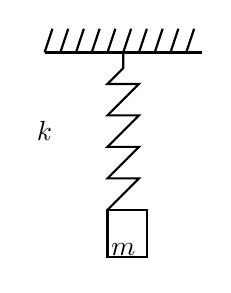
\begin{tikzpicture}

		    % Festes Lager (Decke)
		    \draw[thick] (-1, 4) -- (1, 4);
		        \draw[thick] (-0.9, 4.3) -- (-1.0, 4);
			    \draw[thick] (-0.7, 4.3) -- (-0.8, 4);
			        \draw[thick] (-0.5, 4.3) -- (-0.6, 4);
				    \draw[thick] (-0.3, 4.3) -- (-0.4, 4);
				        \draw[thick] (-0.1, 4.3) -- (-0.2, 4);
					    \draw[thick] (0.1, 4.3) -- (0.0, 4);
					        \draw[thick] (0.3, 4.3) -- (0.2, 4);
						    \draw[thick] (0.5, 4.3) -- (0.4, 4);
						        \draw[thick] (0.7, 4.3) -- (0.6, 4);
							    \draw[thick] (0.9, 4.3) -- (0.8, 4);
							        
								    % Feder (Sägezähne)
								        \draw[thick] (0, 4) -- ++(0, -0.2)
									                 -- ++(-0.2, -0.2) -- ++(0.4, 0) -- ++(-0.4, -0.4)
											                  -- ++(0.4, 0) -- ++(-0.4, -0.4) -- ++(0.4, 0)
													                   -- ++(-0.4, -0.4) -- ++(0.4, 0) -- ++(-0.4, -0.4);
																										                 
																												     % Masse m
																												         \draw[thick] (-0.2, 2.0) rectangle (0.3, 1.4);
																													     \node at (0, 1.5) {$m$};

																													         % Federkonstante k Beschriftung
																														     \node at (-1.0, 3) {$k$};
																														         
	\end{tikzpicture}
		\end{wrapfigure}
		Die Kraft einer Feder wirkt einer Auslenkung aus der Ruhelage $x_0$ entgegen und ist proportional zu dieser. Also ist die Kraft F, die die Feder auf eine Masse m an der Feder aus\"ubt:
		\begin{equation}
			F = -k\cdot(x-x_0)
		\end{equation}
		Dabei ist k die Federkonstante.
	\end{exampleblock}
\end{frame}
\begin{frame}
	\begin{exampleblock}{}
		Die Kraft ist nach dem 1. Newton'schen Axiom $m\cdot a = m\cdot\frac{d^2x}{dt^2}=m\cdot \ddot{x}$, wobei a die Beschleunigung ist. So lautet dann die Dgl.
		\begin{equation}
			m\cdot \ddot{x} = -k\cdot x
		\end{equation}
		wenn Als Ruhelage, der Einfachheit halber, $x_0=0$ gew\"ahlt wird. Das charakteristische Polynom ergibt dann:
		\begin{equation}
			m\cdot\lambda^2 = -k \Rightarrow \lambda = \pm \sqrt{\frac{k}{m}}\cdot i
		\end{equation}
		Damit haben wir Fall 3 und Die L\"osung ist:
		\begin{equation}
			x(t) = C_1\cdot \cos\left(\sqrt{\frac{k}{m}}\cdot t\right) + C_2\cdot \sin\left(\sqrt{\frac{k}{m}}\cdot t\right)
		\end{equation}
		\"Ublicherweise ben\"otigt es dann noch Randbedingungen, beziehungsweise Anfangsbedingungen, um die Konstanten zu bestimmen.
	\end{exampleblock}
\end{frame}
\subsection{Gew\"ohnliche inhomogene Differenzialgleichungen 2. Ordnung}
\begin{frame}
\frametitle{L\"osung inhomogener Dgln.}
	Inhomogene Dgln. werden in 2 Schritten gel\"ost. Zuerst wird die homogene Dgl. gel\"ost und dann die inhomogene Dgl. Je nach Inhomogenit\"at g(x) wird dann ein Ansatz gew\"ahlt(s=sin, c=cos):\\
\begin{tabular}{c|c} 
Inhomogenität $g$ & Ansatz für $y_p$ \\
\hline$b e^{\alpha x}$ & $a e^{\alpha x}x^r$ \\
\hline$b_0+b_1 x+\ldots+b_m x^m$ & $a_0+a_1 x+\ldots+a_m x^m$ \\
	\hline$p_1(x) \sin (\beta x)+p_2(x) \cos (\beta x)$ & $[q_1(x)\sin (\beta x)+ q_2(x)\cos (\beta x)] x^r$ \\
	\hline$e^{\alpha x}\left[p_1(x) s(\beta x)+p_2(x) c(\beta x)\right]$ & $e^{\alpha x}\left[ q_1(x)s(\beta x)+ q_2(x)c(\beta x)\right]x^r$ \\
\hline$e^{\alpha x} p(x)$ & $e^{\alpha x} q(x) x^r$ \\
	Polynom $p_i$ mit Grad $m_i, i\in[1; 2]$ & Polynom $q_i$ mit Grad $max[m_1;m_2]$
\end{tabular}

Tabelle 5.1: Übersicht über mögliche Ansätze zur Berechnung einer partikulären Lösung.
Sind $\alpha$, $\pm i\cdot\beta$ oder $\alpha\pm i\cdot\beta$ Nullstelleen des charakteristischen Polynoms ist r gleich der Vielfachheit der Nullstellen zu setzen, sonst ist r=0 zu setzen. Wenn in der Inhomogenit\"at $\alpha$ und$ \beta$ Vorkommen, muss $\alpha\pm i\cdot\beta$ eine Nullstelle des charakteristischdn Polynoms sein, um $r\neq 0$ zu setzen. 
\end{frame}
\begin{frame}
	\begin{exampleblock}{Getriebener harmonischer Oszillator}
		Wir betrachten wieder den harmonischen Oszillator und ber\"ucksichtigen diesmal die Schwerkraft, also f\"ugen die Inhomogenit\"at $m\cdot g$ hinzu. Damit lautet die Dgl.:
		\begin{equation}
			m\cdot\ddot x + k\cdot x = m\cdot g
		\end{equation}
		Wir machen den Ansatz $y_p=c$. Da die homogene L\"osung eingesetzt verschwindet, bleibt:
		\begin{equation}
			k\cdot c = m\cdot g \Rightarrow c = \frac{m\cdot g}{k}
		\end{equation}

		Die vollst\"andige L\"osung aus homogener und Partikul\"arl\"osung lautet damit:
		\begin{equation}
			x(t) = C_1\cdot \cos\left(\sqrt{\frac{k}{m}}\cdot t\right) + C_2\cdot \sin\left(\sqrt{\frac{k}{m}}\cdot t\right) + \frac{m\cdot g}{k}
		\end{equation}
	\end{exampleblock}
\end{frame}
\begin{frame}
	\begin{exampleblock}{Noch ein etwas schwereres Beispiel}
		\begin{equation}
			y''-4\cdot y'+3y=3\cdot x^2-5\cdot x+4
		\end{equation}
		Die Nullstellen des charakteristischen Polynoms sind 1 und 3. Damit lautet die homogene L\"osung: $y_h(x)=c_1\cdot e^x+c_2\cdot e^{3\cdot x}$. Die Inhomogenit\"at ist ein Polynom 2. Grades, deshalb w\"ahlen wir den Ansatz: $y_p(x)=a\cdot x^2+b\cdot x+c$.
		\begin{equation}
			y_p'(x)=2\cdot a\cdot x+b
		\end{equation}
		\begin{equation}
			y_p''(x)=2\cdot a
		\end{equation}
		Eingesetzt ergibt das:
		\begin{equation}
			2\cdot a - 8\cdot a\cdot x-4\cdot b+3a\cdot x^2+3b\cdot x+3c = 3\cdot x^2-5\cdot x+4
		\end{equation}
	\end{exampleblock}
\end{frame}
\begin{frame}
	\begin{exampleblock}{}
		\begin{equation}
			3a\cdot x^2+(3b-8)x+(2a-4b+3c)=3\cdot x^2-5\cdot x+4
		\end{equation}
		Koeffizientenvergleich ergibt f\"ur $x^2$:
		\begin{equation}
			3a=3
		\end{equation}
		\begin{equation}
			x: 3b-8=-5
		\end{equation}
		\begin{equation}
			x^0: 2a-4b+3c=4
		\end{equation}
		\begin{equation}
			\Rightarrow a=1; b=1; c=2
		\end{equation}
		Damit lautet die vollst\"andige L\"osung:
		\begin{equation}
		y=c_1\cdot e^x+c_2\cdot e^{3\cdot x}+x^2+x+2
		\end{equation}
	\end{exampleblock}
\end{frame}
\subsection{Partielle Differenzialgleichungen}
\begin{frame}
	\frametitle{Separationsansatz f\"ur partielle Dgln.}
  Liegt eine partielle Differenzialgleichung vor, die keine gemischten Ableitungen beinhaltet kann der Separationsansatz gemacht werden.
	F\"ur eine gesuchte Funktion u(x,y,z) wird ein Produktansatz folgender Art gemacht:
		\begin{equation}
			u(x,y,z) = f(x)\cdot g(y)\cdot h(z)
		\end{equation}
		Eingesetzt in die Dgl., kann dann durch u dividiert werden und es entstehen lauter Br\"uche, die jeweils nur von einer Variable abh\"angen. Dann Geben wir den x-abh\"angigen Term nach links und alle anderen nach rechts. Wenn jetzt beide Seiten f\"ur alle x, y und z gleich sein sollen, dann muss die so entstandene Gleichung konstant sein, also k\"onnen wir beide Seiten gleich einer Konstanten K setzen. So entsteht eine gew\"ohnliche Dgl. in x, die wir mit bekannten Methoden l\"osen k\"onnen.
\end{frame}
\begin{frame}
    Mit der anderen Seite, die von y und Z abh\"angt k\"onnen wir gleich verfahren, indem wir den y-abh\"angigen Term auf die Seite von K geben und wieder beide Seiten gleich einer Konstanten L setzen und die zwei \"ubriggebliebenen gew\"ohnlichen Dgln. mit bereits bekannten Methoden l\"osen. Dieses Verfahren l\"asst sich auf eine beliebige Anzahl Variablen anwenden, solange keine gemischten Ableitungen nach diesen Variablen in der partiellen Dgl. (PDGL) auftreten.
\end{frame}
\begin{frame}
	\frametitle{Typen von PDGLn in der Physik}
	\begin{enumerate}	
		\item Potenzialgleichung oder auch Laplacegleichung
			\begin{equation}
				\Delta U = 0
			\end{equation}
			Zur Errinerung
			\begin{equation}
				\Delta U = div \cdot grad U = \nabla \cdot \nabla U = \left( \frac{\partial^2}{\partial x^2}+\frac{\partial^2}{\partial y^2}+\frac{\partial^2}{\partial z^2}\right)U
			\end{equation}
		\item Wellengleichung
			\begin{equation}
				\Delta U = \frac{1}{c^2}\cdot \frac{\partial^2 U}{\partial t^2}
			\end{equation}
		\item W\"armeleitungs- bzw. Diffusionsgleichung
			\begin{equation}
				\Delta U = \frac{1}{\kappa}\cdot \frac{\partial U}{\partial t}
			\end{equation}
		\item Schr\"odingergleichung
			\begin{equation}
				\left(- \frac{\hbar^2}{2\cdot m} + V(x)\right) \Delta \psi = i\cdot \hbar \cdot \frac{\partial \psi}{\partial t}
			\end{equation}
	\end{enumerate}	
\end{frame}
\begin{frame}
	\begin{exampleblock}{inkompressible Station\"are Str\"omung}
		Die Navier-Stokes - Gleichungen f\"ur kompressible Str\"omung lauten:	
			\begin{equation}
				\rho\cdot \frac{Dv_i}{Dt} = -\frac{\partial p}{\partial x_i} + \frac{\partial}{\partial x_i}\left(\bar{\mu} \nabla \cdot v_i \right) + \frac{\partial}{\partial x_j}\left(2\mu D_{ij}\right)+\rho g_i
			\end{equation}
			Wobei $\bar{\mu}$ die Volumenviskosit\"at (zweite Z\"ahigkeit) $\bar{\mu}(p,T)$, $\mu$ die dynamische Viskosit\"at (Scherviskosit\"at) $\mu(p,T)$, $g_i$ je nach Konvention die Erdbeschleunigung in y- oder in z-Richtung und D die massenfeste Zeitableitung ist (das Koordinatensystem sitzt in Massepartikel), im Gegensatz zur ortsfesten Zeitableitung (Koorinatensystem ist ortsfest bzw. raumfest):
			\begin{equation}
				\frac{D\cdot}{Dt}=\frac{\partial\cdot}{\partial t} + \left(v \cdot \nabla\right)\cdot = \frac{\partial\cdot}{\partial t} + v_k \frac{\partial}{\partial x_k}\cdot
			\end{equation}
	\end{exampleblock}
			\end{frame}
			\begin{frame}
				\begin{exampleblock}{}
			$D_{ij}$ ist der symmetrische Teil des Geschwindigkeitsgradienten:
			\begin{equation}
				\frac{\partial v_j}{\partial x_i}=D_{ij}+\Omega_{ij}
			\end{equation}
			\begin{equation}
				D_{ij}=D_{ji}=\frac{1}{2}\cdot \left(\frac{\partial v_i}{\partial x_j}+\frac{\partial v_j}{\partial x_i}\right), \Omega_{ij}=-\Omega_{ji}=\frac{1}{2}\cdot \left(\frac{\partial v_j}{\partial x_i}-\frac{\partial v_i}{\partial x_j}\right)
			\end{equation}
					F\"ur inkompressible Str\"omungen gilt $\nabla \cdot v=0$ und $\mu=\mu(T)$. Bei station\"arer und auch bei horizontaler Str\"omung  kann der "Kraftterm" $\rho \frac{Dv}{Dt}=0$ gesetzt werden, sowie auch g, da es normal auf die Str\"omungsrichtung steht. Der Druckgradient wird konstant und wir setzen ihn -K. Wenn wir die Str\"omungsrichtung in Z-Richtung annehmen, ist v nicht mehr von z abh\"angig. Dann erhalten wir diese Gleichung:
			\begin{equation}
				\left(\frac{\partial^2}{\partial x^2}+\frac{\partial^2}{\partial y^2}\right)v = -\frac{K}{\mu}
			\end{equation}
	\end{exampleblock}
\end{frame}
\begin{frame}
	\begin{exampleblock}{}
		Diese Gleichung l\"osen wir jetzt mit dem Separaionsansatz. Gemischte Ableitungen treten nicht auf, also k\"onnen wir den Produktansatz w\"ahlen:
		\begin{equation}
			v(x, y)=X(x)\cdot Y(y)
		\end{equation}
		eingesetzt in die homogene PDGl. erhalten wir:
		\begin{equation}
			X"\cdot Y+X\cdot Y"= 0\bigg|:\left(X\cdot Y\right)
		\end{equation}
		\begin{equation}
			\frac{X"}{X}\equiv -\frac{Y"}{Y}=C
		\end{equation}
		wir bekommen zwei gew\"ohnliche Dgln
		\begin{equation}
			\frac{X"}{X}=C^2, \frac{Y"}{Y}=-C^2
		\end{equation}
		\begin{equation}
			X=A_1\cdot \sinh\left(C\cdot x\right)+A_2\cdot \cosh\left(C\cdot x\right), Y=B_1\cdot \sin\left(C\cdot x\right)+B_2\cdot \cos\left(C\cdot x\right)
		\end{equation}
	\end{exampleblock}
\end{frame}
\begin{frame}
	\begin{exampleblock}{}
		Jetzt l\"osen wir noch die inhomogene Gleichung. Die zweite Ableitung von v ergibt eine Konstante. Ein Polynom 2. Grades erf\"ullt genau diese Eigenschaft: 
		\begin{equation}
			v = D\cdot x^2 + E\cdot y^2
		\end{equation}
		eingesetzt erhalten wir:
		\begin{equation}
			2\cdot D+2\cdot E=-\frac{K}{\mu}
		\end{equation}
		\begin{equation}
			E=-D-\frac{K}{2\cdot\mu}
		\end{equation}
		Hier ben\"otigen wir noch Randbedingungen um die zweite Konstante zu bestimmen.
	\end{exampleblock}
\end{frame}
\begin{frame}
	\begin{exampleblock}{Die W\"armeleitungsgleichung}
		Wir leiten sie zun\"achst her. Die W\"armemenge Q bekommen wir aus der Temperatur folgenderma{\ss}en:
		\begin{equation}
			Q =  c\cdot m\cdot \Delta T
		\end{equation}
		c ist die spezifische W\"armekapazit\"at, m die Masse und $\Delta$ ist hier ein Delta und nicht der Laplaceoperator. In einem d\"unnen Stab mit Querschnittsfl\"ache A k\"onnen wir die Masse m so asdr\"ucken
		\begin{equation}
			m = \int \rho\cdot A  dx
		\end{equation}
		So k\"onnen wir dann f\"ur den W\"armestrom schreiben:
		\begin{equation}
			\dot{Q} = c\cdot\int \rho\cdot A  dx\cdot  \frac{dT}{dt} \big| \frac{d}{dx}
		\end{equation}
		\begin{equation}
			\frac{\dot{Q}}{dx} = c\cdot\rho\cdot A  \cdot \frac{dT}{dt}
		\end{equation}
	\end{exampleblock}
\end{frame}
\begin{frame}
	\begin{exampleblock}{}
		Das Fourier'sche W\"armeleitgesetz besagt, dass der W\"armestrom proportional zum Temperaturunterschied und zur Fl\"ache ist und indirekt proportional zur Entfernung ist.
		\begin{equation}
			\dot{Q} = -\lambda\cdot A\cdot\frac{dT}{dx}
		\end{equation}
		$\lambda$ ist hier die W\"armeleitf\"ahigkeit oder W\"armeleitkoeffizient.
	Eingesetzt in die vorige Gleichung erhalten wir, wenn wir noch mit einem negativen Vorzeichen ber\"ucksichtigen, dass es sich eigentlich um einen W\"armeverlust handelt:
	\begin{equation}
	\lambda\cdot A\cdot\frac{\partial^2T}{\partial x^2}=c\cdot\rho\cdot A  \cdot \frac{\partial T}{\partial t}
	\end{equation}
	Nach einer Umstellung und k\"urzen von A erhalten wir:	
		\begin{equation}
			\frac{\partial T}{\partial t}=\frac{\lambda}{c\cdot \rho}\frac{\partial ^2T}{\partial x^2}
		\end{equation}
	\end{exampleblock}
\end{frame}
\begin{frame}
	\begin{exampleblock}{}
		Um die W\"armeleitungsgleichung f\"ur alle Raumdimensionen zu erhalten betrachten wir die Bilanz in jeder Raumrichtung und summieren. So erhalten wir:
		\begin{equation}
			\dot{T}=\frac{\lambda}{c\cdot \rho}\Delta T
		\end{equation}
    $\Delta$ ist jetzt der Laplaceoperator.
		Wenn wir den Vorfaktor als Konstante a schreiben und statt der Temperatur die Stoffkonzentration u einsetzen erhalten wir die Diffusionsgleichung.
		\begin{equation}
			\dot{u}=a\cdot\Delta u
		\end{equation}
	\end{exampleblock}
\end{frame}
\begin{frame}
	\begin{exampleblock}{}
Wir machen wieder den Produktansatz:
		\begin{equation}
			u(x,y,z,t)=X(x)\cdot Y(y)\cdot Z(z)\cdot T(t)
		\end{equation}
		Nach Einsetzen und Division durch XYZT erhalten wir:
		\begin{equation}
			\frac{\dot{T}}{T} \equiv a\cdot\left(\frac{X"}{X}+\frac{Y"}{Y}+\frac{Z"}{Z}\right)=K_1
		\end{equation}
		Wir bekommen f\"ur T:
		\begin{equation}
			T(t)=A_1\cdot e^{K_1\cdot t}
		\end{equation}
		\begin{equation}
			\frac{X"}{X}\equiv \frac{K_1}{a}-\left(\frac{Y"}{Y}+\frac{Z"}{Z}\right)=K_2
		\end{equation}
		\begin{equation}
			X(x)=A_2\sinh\left(\sqrt{K_2}\cdot x\right)+A_3\cosh\left(\sqrt{K_2}\cdot x\right)
		\end{equation}
	\end{exampleblock}
\end{frame}
\begin{frame}
	\begin{exampleblock}{}
		\begin{equation}
			\frac{Y"}{Y}\equiv \frac{K_1}{a}-K_2-\frac{Z"}{Z}=K_3
		\end{equation}
		\begin{equation}
			Y(y)=A_4\sinh\left(\sqrt{K_3}\cdot y\right)+A_5\cosh\left(\sqrt{K_3}\cdot x\right)
		\end{equation}
		\begin{equation}
			Z(z)=A_6\sinh\left(\sqrt{\frac{K_1}{a}-K_2-K_3}\cdot z\right)+A_7\cosh\left(\sqrt{\frac{K_1}{a}-K_2-K_3}\cdot z\right)
		\end{equation}
	\end{exampleblock}
\end{frame}
\section{Fourierreihenentwicklung}
\begin{frame}
	\frametitle{Fourierreihenentwicklung}
	\begin{tikzpicture}[scale=0.9, transform canvas={shift={(2.1cm,-1.8cm)}}] % Skalierung und Verschiebung
        \begin{axis}[
            width=10cm, height=7cm,
            xlabel={$x$},
            ylabel={$f(x)$},
            xmin=-pi, xmax=pi,
            ymin=-1.5, ymax=1.5,
            xtick={-pi, -pi/2, 0, pi/2, pi},
            xticklabels={$-\pi$, $-\frac{\pi}{2}$, $0$, $\frac{\pi}{2}$, $\pi$},
            ytick={-1, 0, 1},
            axis lines=middle,
            samples=1000,
            domain=-pi:pi,
	   legend style={
                at={(0.5,-0.15)},
                anchor=north,
                legend columns=-1,
                /tikz/every even column/.append style={column sep=0.5cm},
                fill=none,
                draw=none
            }, 
            cycle list name=color list
%scale only axis,
            %axis on top,
            %every axis plot/.append style={line width=1pt}
        ]

        \addplot[thick, color=cyan, samples=100] {x < -pi/2 + pi/2 ? -1 : (x > pi/2 + pi/2 ? -1 : 1)};
        \addlegendentry{Funktion}

        \addplot[domain=-pi:pi, samples=100, thick, color=red] {4/pi * sin(deg(x))};
        \addlegendentry{$n=1$}

        \addplot[domain=-pi:pi, samples=100, thick, color=blue] {4/pi * (sin(deg(x)) + (1/3)*sin(deg(3*x)))};
        \addlegendentry{$n=3$}

        \addplot[domain=-pi:pi, samples=100, thick, color=green] {4/pi * (sin(deg(x)) + (1/3)*sin(deg(3*x)) + (1/5)*sin(deg(5*x)))};
        \addlegendentry{$n=5$}

        \addplot[domain=-pi:pi, samples=100, thick, color=orange] {4/pi * (sin(deg(x)) + (1/3)*sin(deg(3*x)) + (1/5)*sin(deg(5*x)) + (1/7)*sin(deg(7*x)))};
        \addlegendentry{$n=7$}

        \addplot[domain=-pi:pi, samples=100, thick, color=purple] {4/pi * (sin(deg(x)) + (1/3)*sin(deg(3*x)) + (1/5)*sin(deg(5*x)) + (1/7)*sin(deg(7*x)) + (1/9)*sin(deg(9*x)))};
        \addlegendentry{$n=9$}

        \end{axis}
    \end{tikzpicture}
\end{frame}
\begin{frame}
	\frametitle{Einschub gerade Funktionen, ungerade Funktionen}
	F\"ur ungerade Funktionen gilt: $f(x)=-f(-x)$ und sie sind punktsymmetrisch bez\"uglich des Ursprungs. Ein Beispiel f\"ur eine ungerade Funktion ist der Sinus:
	\begin{tikzpicture}[scale=0.9]
		\draw[->] (-2*pi,0) -- (2*pi,0) node[right] {$x$};
		\draw[->] (0,-1.5) -- (0,1.5) node[above] {$f(x)$};
		\draw[scale=1,domain=-2*pi:2*pi,smooth,variable=\x,cyan] plot ({\x},{sin(\x r)});
	\end{tikzpicture}

\end{frame}
\begin{frame}
	F\"ur gerade Funktionen gilt: $f(x)=f(x)$ und sie sind spiegelsymmetrisch bez\"uglich der y-Achse (Ordinate). Ein Beispiel f\"ur eine gerade Funktion ist der Cosinus:
	\begin{tikzpicture}[scale=0.9]
		\draw[->] (-2*pi,0) -- (2*pi,0) node[right] {$x$};
		\draw[->] (0,-1.5) -- (0,1.5) node[above] {$f(x)$};
		\draw[scale=1,domain=-2*pi:2*pi,smooth,variable=\x,cyan] plot ({\x},{cos(\x r)});
	\end{tikzpicture}

\end{frame}
\begin{frame}
	\frametitle{Fourierreihenentwicklung}
	Motivation: N\"aherung einer periodischen Funktion durch Winkelfunktionen, bzw. Zerlegung in Frequenzen. Eine andere Betrachtungsweise w\"are Sin und Cos mit den verschiedenen Frequenzen Als Basisvektoren f\"ur einen Vektorraum zu betrachten. Dann w\"are eine Linearkombination dieser Basisvektoren eine eindeutige Darstellung dieser periodischen Funktion.
$$
	f(x)=\frac{\alert{a_0}}{2}+\sum_{n=1}^{\infty}\left(\alert{a_n} \cos (n x)\right)+\sum_{n=1}^{\infty}\left(\alert{b_n} \sin (n x)\right)
$$
Durch Integration von $T$ bis $T+2\pi$ nach x erhalten wir:
$$
\begin{aligned}
&\int_T^{T+2 \pi} f(x) d x  =\frac{a_0}{2} \int_T^{T+2 \pi} d x+\\
	&+\sum_{n=1}^{\infty}\left[a_n \int_T^{T+2 \pi} \cos (n x) d x+b_n \int_T^{T+2 \pi} \sin (n x) d x\right]= \\
\end{aligned}
	$$
\end{frame}
\begin{frame}
	$$
\begin{aligned}
	& =\frac{a_0}{2}(T+2 \pi-T)+\sum_{n=1}^{\infty}\left[a_n\left(\frac{\sin (n x)}{n}\right)_T^{T+2 \pi}+b_n\left(\frac{-\cos (n x)}{n}\right)_T^{T+2 \pi}\right] \\
& =a_0 \pi+\sum_{n=1}^{\infty}\left[a_n\cdot 0-b_n\cdot 0\right] \\
& =a_0 \pi
\end{aligned}
$$
Nach $a_0$ umgeformt bekommen wir:
$$
	\alert{a_0=\frac{1}{\pi} \int_T^{T+2 \pi} f(x) d x}
	$$
\end{frame}
\begin{frame}
	Jetzt m\"ochten wir eine Formel f\"ur $a_n$ bekommen. Wir multiplizieren dazu beide Seiten mit $\cos(mx)$ und integrieren wieder.
	
	$$\int_T^{T+2 \pi} f(x) \cos (m x) d x=\frac{a_0}{2} \int_T^{T+2 \pi} \cos (m x) d x+$$\\ 
	$$+\sum_{n=1}^{\infty} a_n\left[\int_T^{T+2\pi} \cos (n x) \cos (m x) d x\right]+\sum_{n=1}^{\infty} b_n\left[\int_T^{T+2\pi} \sin (n x) \cos (mx) d x\right]$$
	$$
	\begin{aligned}
		&\int_T^{T+2 \pi} f(x) \cos (n x) d x  =\frac{1}{2} \sum_{n=1}^{\infty}\left[a_n \int_T^{T+2 \pi} 2 \cdot \cos ^2(n x) d x\right] \\
		& =\frac{a_n}{2} \int_T^{T+2 \pi}(1+\cos (2 n x)) d x \\
		& =\frac{a_n}{2}\left(x+\frac{\sin (2 n x)}{2 n}\right)_T^{T+2 \pi} \\
		& =\frac{a_n}{2}(2 \pi)=a_n \pi\Rightarrow \alert{a_n=\frac{1}{\pi} \int_T^{T+2 \pi} f(x) \cos (n x) d x}
	\end{aligned}
	$$
	
\end{frame}
\begin{frame}
	 Die Begr\"undung, warum m=n wird ist, dass bei Betrachtung als Skalarprodukt, das Skalaprodukt nur f\"ur gleiche Basisvektoren ungleich 0 wird. Zuguterletzt h\"atten wir noch gerne eine Formel f\"ur $b_n$. Dazu multiplizieren wir beide Seiten mit $\sin(mx)$:
	$$\int_T^{T+2 \pi} f(x) \sin (m x) d x=$$\\ 
	$$=\frac{a_0}{2} \int_T^{T+2 \pi} \sin (m x) d x+\sum_{n=1}^{\infty} a_n\left[\int_T^{T+2 \pi} \cos (n x) \sin (m x) d x\right]+$$\\
	$$+\sum_{n=1}^{\infty} b_n\left[\int_T^{T+2 \pi} \sin (n x) \sin (mx) d x\right]$$
\end{frame}
\begin{frame}
	Die ersten beiden Integrale der rechten Seite verschwinden und es bleibt:
	$$
	\begin{aligned}
		\int_T^{T+2 \pi} f(x) \sin (n x) & d x=\frac{1}{2} \sum_{n=1}^{\infty}\left[b_n \int_T^{T+2 \pi} 2 \cdot \sin ^2(n x) d x\right] \\
		& =\frac{b_n}{2} \int_T^{T+2 \pi}(1-\cos (2 n x)) d x \\
		& =\frac{b_n}{2}\left(x-\frac{\sin (2 n x)}{2 n}\right)_T^{T+2 \pi} \\
		= & \frac{b_n}{2}(2 \pi)=b_n \pi
	\end{aligned}
	$$
	$$
	\Rightarrow \alert{b_n=\frac{1}{\pi} \int_T^{T+2 \pi} f(x) \sin (n x) d x}
	$$
\end{frame}
\begin{frame}
	\begin{exampleblock}{Beispiel: Kippschwingung}
		Wir modellieren eine Kippschwingung mit Periode $2 \pi$ und Werten zwischen $-\pi$ und $\pi$ mithilfe der Funktion
		$$
		g(x)=\left\{\begin{array}{cl}
			x & \text { wenn }-\pi<x \leq \pi \\
			\text { periodisch fortgesetzt } & \text { sonst. }
		\end{array}\right.
		$$

		 $g$ ist stückweise stetig differenzierbar, aber unstetig und (abgesehen von den Unstetigkeitsstellen) eine ungerade Funktion, daher ist $a_n=0$. Wir müssen also nur die Fourierkoeffizienten $b_n$ ermitteln, wobei hier die Partielle Integration zum Ziel f\"uhrt:
		$$
		b_n=\frac{1}{\pi} \int_{-\pi}^\pi \sin (n x) g(x) d x=\frac{1}{\pi} \int_{-\pi}^\pi \sin (n x) x d x = -\frac{2}{n}(-1)^n= \frac{2}{n}(-1)^{n+1} .
		$$
		$$
		\Rightarrow\widetilde{g}(x)=\sum_{n=1}^{\infty} \frac{2(-1)^{n+1}}{n} \sin (n x)
		$$
	\end{exampleblock}
\end{frame}
\begin{frame}
	\frametitle{Eine etwas unkonventionellere Anwendung der Fourieranalyse}
	\begin{center}
	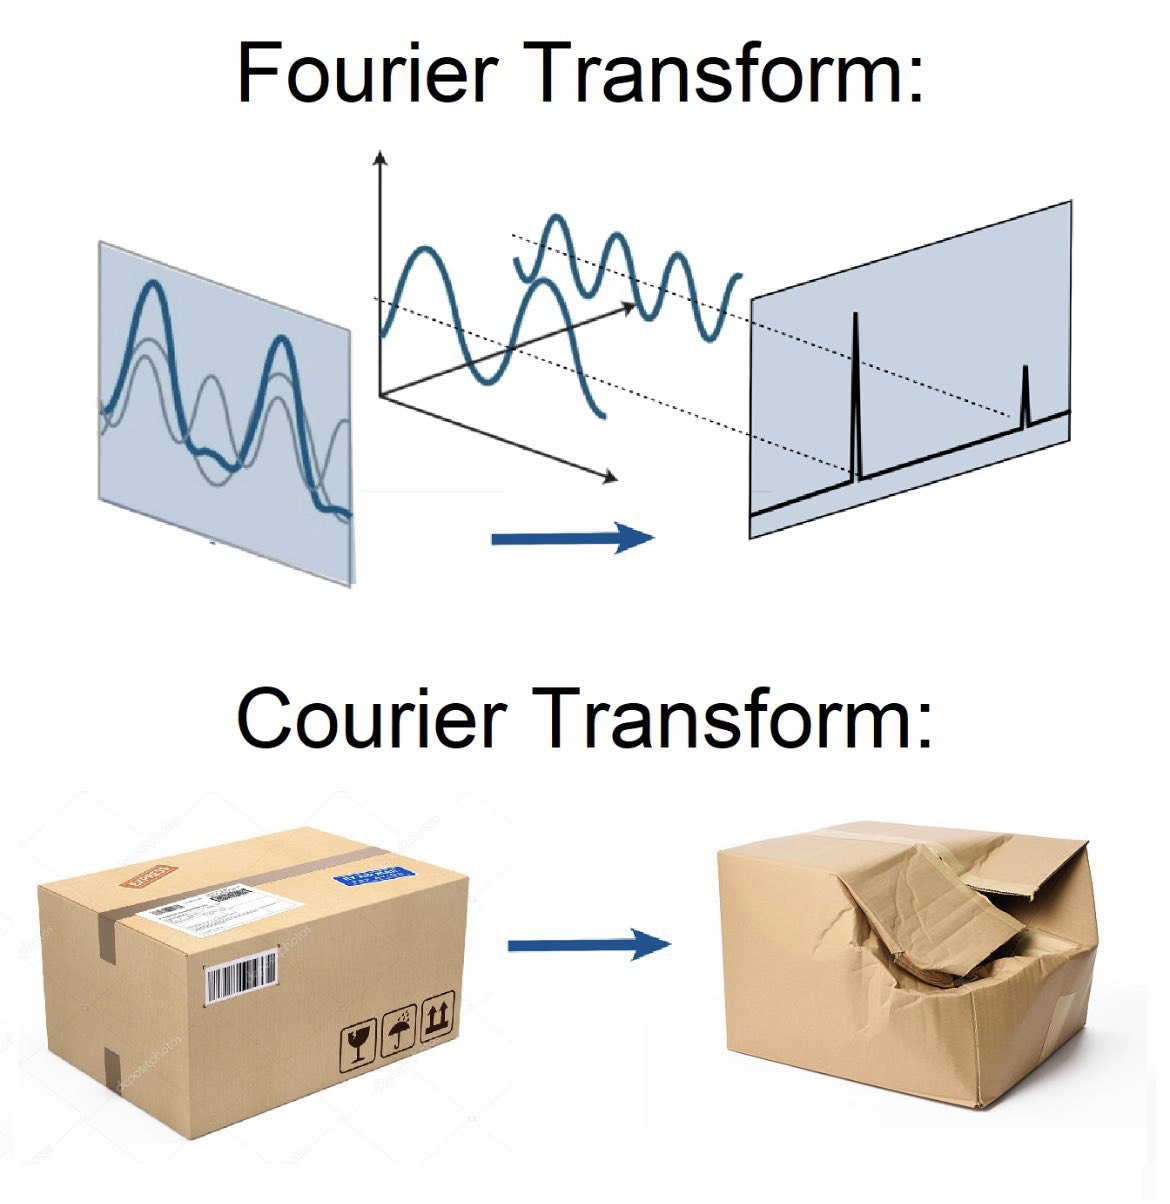
\includegraphics[scale=0.17]{ct}
	\end{center}
\end{frame}
\begin{frame}
		\frametitle{Fragen? Kommentare?}
	\begin{center}
	%\begin{wrapfigure}{l}{0.6\textwidth}
	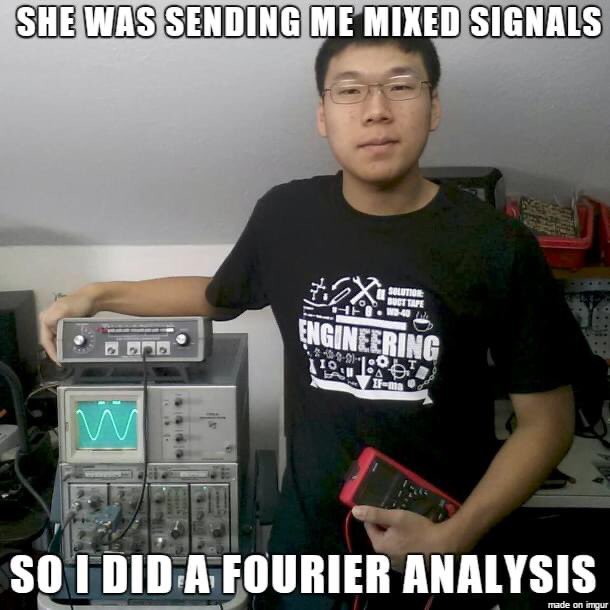
\includegraphics[scale=0.35]{ms}
	%\begin{wrapfigure}
	\end{center}
\end{frame}
\section{Anhang}
		\subsection{inkompressible Str\"omungen}
\begin{frame}
	\frametitle{Inkompressible Str\"omungen}
		Zum Zeitpunkt 0 befindet sich ein Fluidpartikel in der Str\"omung am Ort \textbf{X}(x,y,z), zu einem Zeitpunkt $t>0$ am Ort \textbf{x}(x,y,z). Wir unterscheiden dann bei einer physikalischen Gr\"o{\ss}e b zwischen der massenfesten Zeitabeitung
		\begin{equation}
      \frac{Db}{Dt}=\frac{\partial b(\textbf{X}, t)}{\partial t} \label{mfza}
		\end{equation}
		und der ortsfesten Zeitableitung
		\begin{equation}
      \frac{\partial b}{\partial t}=\frac{\partial b(\textbf{x}, t)}{\partial t} \label{ofza}
		\end{equation}
		Die Teilchengeschwindigkeit v ist dann $\frac{D\textbf{x}}{Dt}$ und die Teilchenbeschleunigung ist dann $\frac{D\textbf{v}}{Dt}$. In Indexschreibweise und unter Verwendung der Einstein'schen Summenkonvention, dass in einem Term \"uber doppelt vorkommende Indizes summiert wird:
		\begin{equation}
			\frac{Dv_i}{Dt}=\frac{\partial v_i}{\partial t} + \frac{\partial v_i}{\partial x_j}\cdot \frac{Dx_j}{Dt} 
		\end{equation}

\end{frame}
\begin{frame}
		\begin{equation}
      \Rightarrow \textbf{a}=\frac{D\textbf{v}}{Dt}=\frac{\partial \textbf{v}}{\partial t}+\left(\textbf{v}\cdot\nabla\right)\textbf{v} \label{mfzat}
		\end{equation}
		Also gilt allgemein f\"ur eine Gr\"o{\ss}e b
		\begin{equation}
			\frac{D\textbf{b}}{Dt}=\frac{\partial \textbf{b}}{\partial t}+\left(\textbf{v}\cdot\nabla\right)\textbf{b}
		\end{equation}
		Die Dehnung eines infinitesimalen Volumens dV w\"ahrend der Bewegung wird durch die Funktionaldeterminante
		\begin{equation}
		\operatorname{det} J(\mathbf{X}, t)=\frac{\partial(x, y, z)}{\partial(X, Y, Z)}=\left\lvert\, \begin{aligned} & \frac{\partial x}{\partial X} \frac{\partial x}{\partial Y} \frac{\partial x}{\partial Z} \\ & \frac{\partial y}{\partial X} \ldots \\ & \ldots\end{aligned}\right\rvert
		\end{equation}

			charakterisiert. $J=\left(\frac{\partial x_i}{\partial X_j}\right)=\left(c_{i j}\right)$ ist dabei die Jacobimatrix der Transformation.
\end{frame}
\begin{frame}
	Der laplace'sche Entwicklungssatz f\"ur Determinanten l\"asst sich auf folgende Weise schreiben:
	\begin{equation}
		\operatorname{det}J = \sum_{k=1}^3 c_{ik}\cdot \alpha_{ik}, \alpha_{ik}=(-1)^{i+k} \operatorname{det}J_{ik}
	\end{equation}
	hier f\"ur die Entwicklung nach der i-ten Zeile, f\"ur beliebiges aber festes i zwischen 1 und 3. Dabei sind $c_{ik}$ die Elemente der Jacobimatrix und $\alpha_{ik}$ die algebraischen Komplemente der i-en Zeile und k-ten Spalte und det $J_{ik}$ jene Unterdeterminanten (Minoren), die sich jeweils duech Streichen der i-ten Zeile und k-ten Spalte ergeben.
	\begin{equation}
		\sum_{k=1}^3 c_{ik}\cdot \alpha_{jk}=\delta_{ij}\operatorname{det}J
	\end{equation}
		$$
		\delta_{ij}=\left\{\begin{array}{cl}
			1 & \text { wenn }i = j \\
			0 & \text { sonst. }
		\end{array}\right.
		$$

	Das k\"onnen wir f\"ur die Ableitung der Funktionaldeterminante verwenden
\end{frame}
\begin{frame}
	\begin{equation}
		\frac{d\operatorname{det}J}{dx}=\sum_{i=1}^3\sum_{j=1}^3\underbrace{\frac{\partial\operatorname{det}J}{\partial c_{ij}}}_{\alpha_{ij}}\frac{dc_{ij}}{dx}
	\end{equation}
	\begin{equation}
		\Rightarrow \frac{D\operatorname{det}J}{Dt}=\sum_{i=1}^3\sum_{j=1}^3\alpha_{ij}\frac{Dc_{ij}}{dt}=\sum_{i=1}^3\sum_{k=1}^3\underbrace{\sum_{j=1}^3c_{kj}\alpha_{ij}}_{\delta_{ki}\operatorname{det} J}\frac{\partial v_i}{\partial x_k}=\operatorname{det} J\underbrace{\sum_{i=1}^3\frac{\partial v_i}{\partial x_i}}_{\nabla\cdot v}
	\end{equation}
	Mit
	\begin{equation}
		\frac{Dc_{ij}}{Dt}=\frac{D}{Dt}\left(\frac{\partial x_i}{\partial X_j}\right)=\frac{\partial v_i}{\partial X_j}=\sum_{k=1}^3\frac{\partial v_i}{\partial x_k}\underbrace{\frac{\partial x_k}{\partial X_j}}_{c_{kj}}
	\end{equation}
	Da bei inkompressiblen Str\"omungen die Str\"omung keine Volumendehnung erf\"ahrt, muss die Zeitableitung der Funktionaldeterminante verschwinden. Damit das f\"ur alle beliebigen Funktionaldeterminanten der Fall ist muss im Produkt $\nabla\cdot v=0$ sein. 
\end{frame}
		\subsection{Navier-Stokes - Gleichungen}
\begin{frame}
	\frametitle{Herleitung der Navier-Stokes - Gleichungen}
	Diese sind im Prinzip Bewegungsgleichungen f\"ur ein viskoses, Newton'sches Fluid. Diese k\"onnen wir aus der Impulserhaltung in integraler Form herleiten:
	\begin{equation}
		\frac{D}{Dt}\int_V \rho v_i dV=\int_{\partial V}\sigma_{ji}n_j dO+\int \rho g_i dV + K_i
	\end{equation}
		Die resultierende Kraft ergipt sich dabei aus dem an der Oberfl\"ache wirkenden Spannungsvektor $\sigma_{ji}\cdot n_j$, wobei $\sigma_{ji}$ der Spannunstensor ist, der Erdanziehungskraft und einer Kraft K, die ein umstr\"omter K\"orper im Volumen V auf die Str\"omung aus\"ubt. Mithilfe des Gau{\ss}'schen Satzes k\"onnen wir den Spannungvektor umschreiben.
		\begin{equation}
			\int_V \rho \frac{Dv_i}{Dt} dV=\int_{V}\frac{\partial \sigma_{ji}}{\partial x_j} +\rho g_i dV
		\end{equation}
    Die Ableitung au{\ss}erhalb des Integrals im linken Term ist nicht von Vorne herein einfach nur die Ableitung der Geschwindigkeit. Wir ben\"otigen dazu das Transporttheorem \eqref{tt}, das im Sinne der \"Ubersicht am Ende an die Herleitung noch hergeleitet wird.
\end{frame}
\begin{frame}
	Auch haben wir den Bereich fester K\"orper ausgeschlossen, da wir in differenzieller Form nur einen lokalen Bereich betrachten und K=0 gesetzt. Da der Zusammenhang f\"ur ein beliebigesVolumen gelten soll:
	\begin{equation}
			\rho \frac{Dv_i}{Dt} =\frac{\partial \sigma_{ji}}{\partial x_j} +\rho g_i 
	\end{equation}
	\"Ublicherweise wird der Spannungstensor in einen Tensor der inneren Reibspannungen $\left(\sigma_{ji}'\right)$ und einen Anteil $p\delta_{ij}$, der vom Druck herr\"uhrt, aufgespalten:
	\begin{equation}
		\sigma_{ji}=\sigma_{ji}'-p\delta_{ij}
	\end{equation}
	\begin{equation}
		\rho \frac{Dv_i}{Dt} =-\frac{\partial p}{\partial x_i}+\frac{\partial \sigma_{ji}'}{\partial x_j} +\rho g_i 
	\end{equation}
	Um die Navier-Stokes - Gleichungn zu erhalten ben\"otigen wir einen Ausdruck f\"ur den Reibspannungstensor.
\end{frame}
\begin{frame}
	Die Stokes'schen Postulate f\"ur ein viskoses, Stokes'sches Fluid lauten:
	\begin{enumerate}
		\item $\sigma_{ij}$ ist eine stetige Funktion von $D_{ij}$, unabh\"angig von anderen kinematischen Gr\"o{\ss}en,
		\item $\sigma_{ij}$ h\"angt nicht explizit von der r\"aumlichen Position \textbf{x} ab.
		\item es existiert keine ausgezeichnete Richtung im Raum (Isotropie)
		\item falls $D_{ij}=0$, dann gelte $\sigma_{ij}=-p\delta_{ij}$.
	\end{enumerate}
	Die mathematische \"Ubersetzung von 1 und 2 ist $\sigma=f\left(D\right)$.\\
	3 dr\"uckt sich durch $O\sigma O^{-1}=f\left(ODO^{-1}\right)$ f\"ur alle orthogonalen Transformationsmatrizen O aus.
\end{frame}
\begin{frame}
	1-4 f\"uhren auf die nichtlineare quadratische Relation
	\begin{equation}
		\sigma_{ij}=\alpha\delta_{ij}+\beta D_{ij}+\gamma D_{ik}D_{kj}
	\end{equation}
	Die griechischen Variablen sind skalare Funktionen von $I_1, I_2$ und $I_3$, den Hauptinvarianten von D. Diese sind die Koeffizienten im charakteristischen Polynom
	\begin{equation}
		p_D(\lambda)=\operatorname{det}(\lambda-D)=\lambda^3-I_1 \lambda^2+I_2 \lambda-I_3=0
	\end{equation}
	Wenn wir fordern, dass $\sigma$ linear von D abh\"angt dann nennen wir ein solches Fluid ein Newton'sches Fluid.Wir erhalten dann f\"ur $\sigma$
	\begin{equation}
		\sigma_{ij}=\sigma_{ji}=\left(-p+\bar{\mu}\nabla\cdot\textbf{v}\right)\delta_{ij}+2\mu D_{ij}
	\end{equation}
\end{frame}
\begin{frame}
	und $\sigma'$
	\begin{equation}
		\sigma_{ij}'=\sigma_{ji'}=\bar{\mu}\nabla\cdot\textbf{v}\delta_{ij}+2\mu D_{ij}
	\end{equation}
	Eingesetzt in die Bewegungsgleichung erhalten wir die lang ersehnten Navier-Stokes - Gleichungen
	\begin{equation}
		\rho \frac{Dv_i}{Dt} =-\frac{\partial p}{\partial x_i}+\frac{\partial}{\partial x_i} \left(\bar{\mu}\nabla\cdot\textbf{v}\right)+\frac{\partial}{\partial x_j}\left(2\mu D_{ij}\right) +\rho g_i 
	\end{equation}
	F\"ur ein  perfektes (reibungsfreies) Fluid erhalten wir die Eulergleichungen
	\begin{equation}
		\rho \frac{Dv_i}{Dt} =-\frac{\partial p}{\partial x_i} +\rho g_i 
	\end{equation}
	F\"ur ein nicht newton'sches Fluid mit konstanten Stoffwerten $\rho,\mu=$const. bekommen wir
	\begin{equation}
		\frac{Dv_i}{Dt} =-\frac{1}{\rho}\frac{\partial p}{\partial x_i}+\nu \frac{\partial^2 v_i}{\partial x_j^2} +\rho g_i 
	\end{equation}
	deren station\"are Variante wir mit dem Separationsansatz l\"osen k\"onnen, wobei $\nu=\frac{\mu}{\rho}$ ist.
\end{frame}
		\subsection{Transporttheorem}
\begin{frame}
	\frametitle{Einschub Transporttheorem}
  Sei $V(t)$ ein mit der Strömung massenfest mitbewegtes Kontrollvolumen und $b(\mathbf{x}, t)$ eine beliebige Feldgröße. Dann gilt für die Transformation von Bereichsintegralen:
$$
\int_V b(\mathbf{x}, t) \mathrm{d} V=\int_{V_0} b(\mathbf{X}, t) \underbrace{|\operatorname{det} J(\mathbf{X}, t)| \mathrm{d} V_0}_{\mathrm{d} V}, \quad V_0=V(0)=\text { const. }
$$

  Die massenfeste Zeitableitung dieses Ausdrucks ist unter Verwendung von ~\eqref{mfza},  ~\eqref{ofza} und \eqref{mfzat} gegeben durch
$$
\begin{aligned}
\frac{\mathrm{D}}{\mathrm{D} t} \int_V b \mathrm{~d} V & =\int_{V_0}(b \underbrace{\frac{\mathrm{D}|\operatorname{det} J|}{\mathrm{D} t}}_{|\operatorname{det} J| \nabla \cdot \mathbf{v}}+|\operatorname{det} J| \frac{\mathrm{D} b}{\mathrm{D} t}) \mathrm{d} V_0\\
  & =\int_{V_0}\left(\frac{\mathrm{D} b}{\mathrm{D} t}+b \nabla \cdot \mathbf{v}\right)|\operatorname{det} J| \mathrm{d} V_0 \\
& =\int_V\left(\frac{\mathrm{D} b}{\mathrm{D} t}+b \nabla \cdot \mathbf{v}\right) \mathrm{d} V=\int_V\left(\frac{\partial b}{\partial t}+\nabla \cdot(b \mathbf{v})\right) \mathrm{d} V
\end{aligned}
$$

\end{frame}
\begin{frame}
  Bemerkenswert ist folgende Relation, die mit Hilfe des Transporttheorems für eine beliebige Feldgröße $b$ angegeben werden kann:
$$
  \frac{\mathrm{D}}{\mathrm{D} t} \int_V \rho b \mathrm{~d} V=\int_V(\rho \frac{\mathrm{D} b}{\mathrm{D} t}+b \underbrace{\frac{\mathrm{D} \rho}{\mathrm{D} t}}_{-\rho \nabla \cdot \mathbf{v}}+\rho b \nabla \cdot \mathbf{v}) \mathrm{d} V=\int_V \rho \frac{\mathrm{D} b}{\mathrm{D} t} \mathrm{~d} V . \label{tt}
$$
 die wir f\"ur die Herleitung der Bewegungsgleichung ben\"otigen.
\end{frame}
%\begin{frame}
%	\frametitle{Lists}
%	\framesubtitle{Bullet Points and Numbered Lists} % Optional subtitle
%	
%	\begin{itemize}
%		\item Lorem ipsum dolor sit amet, consectetur adipiscing elit
%		\item Aliquam blandit faucibus nisi, sit amet dapibus enim tempus
%		\begin{itemize}
%			\item Lorem ipsum dolor sit amet, consectetur adipiscing elit
%			\item Nam cursus est eget velit posuere pellentesque
%		\end{itemize}
%		\item Nulla commodo, erat quis gravida posuere, elit lacus lobortis est, quis porttitor odio mauris at libero
%	\end{itemize}
%	
%	\bigskip % Vertical whitespace
%	
%	\begin{enumerate}
%		\item Nam cursus est eget velit posuere pellentesque
%		\item Vestibulum faucibus velit a augue condimentum quis convallis nulla gravida 
%	\end{enumerate}
%\end{frame}
%
%%------------------------------------------------
%
%\subsection{Blocks}
%
%\begin{frame}
%	\frametitle{Blocks of Highlighted Text}
%	
%	\begin{block}{Block Title}
%		Lorem ipsum dolor sit amet, consectetur adipiscing elit. Integer lectus nisl, ultricies in feugiat rutrum, porttitor sit amet augue.
%	\end{block}
%	
%	\begin{exampleblock}{Example Block Title}
%		Aliquam ut tortor mauris. Sed volutpat ante purus, quis accumsan.
%	\end{exampleblock}
%	
%	\begin{alertblock}{Alert Block Title}
%		Pellentesque sed tellus purus. Class aptent taciti sociosqu ad litora torquent per conubia nostra, per inceptos himenaeos.
%	\end{alertblock}
%	
%	\begin{block}{} % Block without title
%		Suspendisse tincidunt sagittis gravida. Curabitur condimentum, enim sed venenatis rutrum, ipsum neque consectetur orci.
%	\end{block}
%\end{frame}
%
%%------------------------------------------------
%
%\subsection{Columns}
%
%\begin{frame}
%	\frametitle{Multiple Columns}
%	\framesubtitle{Subtitle} % Optional subtitle
%	
%	\begin{columns}[c] % The "c" option specifies centered vertical alignment while the "t" option is used for top vertical alignment
%		\begin{column}{0.45\textwidth} % Left column width
%			\textbf{Heading}
%			\begin{enumerate}
%				\item Statement
%				\item Explanation
%				\item Example
%			\end{enumerate}
%		\end{column}
%		\begin{column}{0.5\textwidth} % Right column width
%			Lorem ipsum dolor sit amet, consectetur adipiscing elit. Integer lectus nisl, ultricies in feugiat rutrum, porttitor sit amet augue. Aliquam ut tortor mauris. Sed volutpat ante purus, quis accumsan dolor.
%		\end{column}
%	\end{columns}
%\end{frame}
%
%%------------------------------------------------
%
%\section{Table and Figure Examples}
%
%\subsection{Table}
%
%\begin{frame}
%	\frametitle{Table}
%	\framesubtitle{Subtitle} % Optional subtitle
%	
%	\begin{table}
%		\begin{tabular}{l l l}
%			\toprule
%			\textbf{Treatments} & \textbf{Response 1} & \textbf{Response 2}\\
%			\midrule
%			Treatment 1 & 0.0003262 & 0.562 \\
%			Treatment 2 & 0.0015681 & 0.910 \\
%			Treatment 3 & 0.0009271 & 0.296 \\
%			\bottomrule
%		\end{tabular}
%		\caption{Table caption}
%	\end{table}
%\end{frame}
%
%%------------------------------------------------
%
%%\subsection{Figure}
%%
%%\begin{frame}
%%	\frametitle{Figure}
%%	
%%	\begin{figure}
%%		
\includegraphics[width=0.8\linewidth]{creodocs_logo.pdf}
%%		\caption{Creodocs logo.}
%%	\end{figure}
%%\end{frame}
%%
%%%------------------------------------------------
%%
%%\section{Mathematics}
%%
%%\begin{frame}
%%	\frametitle{Definitions \& Examples}
%%	
%%	\begin{definition}
%%		A \alert{prime number} is a number that has exactly two divisors.
%%	\end{definition}
%%	
%%	\smallskip % Vertical whitespace
%%	
%%	\begin{example}
%%		\begin{itemize}
%%			\item 2 is prime (two divisors: 1 and 2).
%%			\item 3 is prime (two divisors: 1 and 3).
%%			\item 4 is not prime (\alert{three} divisors: 1, 2, and 4).
%%		\end{itemize}
%%	\end{example}
%%	
%%	\smallskip % Vertical whitespace
%%	
%%%	You can also use the \texttt{theorem}, \texttt{lemma}, \texttt{proof} and \texttt{corollary} environments.
%%\end{frame}
%
%%------------------------------------------------
%
%%\begin{frame}
%%	\frametitle{Theorem, Corollary \& Proof}
%%	
%%	\begin{theorem}[Mass--energy equivalence]
%%		$E = mc^2$
%%	\end{theorem}
%%	
%%	\begin{corollary}
%%		$x + y = y + x$
%%	\end{corollary}
%%	
%%	\begin{proof}
%%		$\omega + \phi = \epsilon$
%%	\end{proof}
%%\end{frame}
%
%%------------------------------------------------
%
%%\begin{frame}
%%	\frametitle{Equation}
%%
%%	\begin{equation}
%%		\cos^3 \theta =\frac{1}{4}\cos\theta+\frac{3}{4}\cos 3\theta
%%	\end{equation}
%%\end{frame}
%%
%%%------------------------------------------------
%%
%%\begin{frame}[fragile] % Need to use the fragile option when verbatim is used in the slide
%%	\frametitle{Verbatim}
%%	
%%	\begin{example}[Theorem Slide Code]
%%		\begin{verbatim}
%%			\begin{frame}
%%				\frametitle{theorem}
%%				\begin{theorem}[Mass--energy equivalence]
%%					$E = mc^2$
%%				\end{theorem}
%%		\end{frame}\end{verbatim} % Must be on the same line
%%	\end{example}
%%\end{frame}
%%
%%%------------------------------------------------
%%
%%\begin{frame}
%%	Slide without title.
%%\end{frame}
%
%%------------------------------------------------
%\section{Referencing}
%
%\begin{frame}
%	\frametitle{Citing References}
%	
%%	An example of the \texttt{\textbackslash cite} command to cite within the presentation:
%	
%	\bigskip % Vertical whitespace
%	
%	%This statement requires citation \cite{p1,p2}.
%\end{frame}
%
%%------------------------------------------------
%
%\begin{frame} % Use [allowframebreaks] to allow automatic splitting across slides if the content is too long
%	\frametitle{References}
%	
%	\begin{thebibliography}{99} % Beamer does not support BibTeX so references must be inserted manually as below, you may need to use multiple columns and/or reduce the font size further if you have many references
%		\footnotesize % Reduce the font size in the bibliography
%		\setbeamertemplate{bibliography item}[text]
%		\bibitem[Smith, 2022]{p1}
%			John Smith (2022)
%			\newblock Publication title
%			\newblock \emph{Journal Name} 12(3), 45 -- 678.
%			
%		\bibitem[Kennedy, 2023]{p2}
%			Annabelle Kennedy (2023)
%			\newblock Publication title
%			\newblock \emph{Journal Name} 12(3), 45 -- 678.
%	\end{thebibliography}
%\end{frame}
%
%%----------------------------------------------------------------------------------------
%%	ACKNOWLEDGMENTS SLIDE
%%----------------------------------------------------------------------------------------
%
%\begin{frame}
%	\frametitle{Acknowledgements}
%	
%	\begin{columns}[t] % The "c" option specifies centered vertical alignment while the "t" option is used for top vertical alignment
%		\begin{column}{0.45\textwidth} % Left column width
%			\textbf{Smith Lab}
%			\begin{itemize}
%				\item Alice Smith
%				\item Devon Brown
%			\end{itemize}
%			\textbf{Cook Lab}
%			\begin{itemize}
%				\item Margaret
%				\item Jennifer
%				\item Yuan
%			\end{itemize}
%		\end{column}		
%		\begin{column}{0.5\textwidth} % Right column width
%			\textbf{Funding}
%			\begin{itemize}
%				\item British Royal Navy
%				\item Norwegian Government
%			\end{itemize}
%		\end{column}
%	\end{columns}
%\end{frame}

%----------------------------------------------------------------------------------------
%	CLOSING SLIDE
%----------------------------------------------------------------------------------------

%\begin{frame}[plain] % The optional argument 'plain' hides the headline and footline
%	\begin{center}
%		{\Huge The End}
%		
%		\bigskip\bigskip % Vertical whitespace
%		
%		{\LARGE Questions? Comments?}
%	\end{center}
%\end{frame}

%----------------------------------------------------------------------------------------

\end{document} 
